\section{Prediction of Likes and Reposts in Video Selfies}
With the recent advances in software frameworks and tools that help in designing neural networks \cite{Bastien-Theano-2012} \cite{bergstra+al:2010-scipy} , training a neural network to learn a pattern in higher dimensional abstraction is easier. Because we found a decent correlation in the initial Support vector regression between Sentibank class probability distribution and repost/like distribution, we chose to use the 2089 dimensional ANP probability vectors that arise from Sentibank analysis as input random variable to our network. Before using them as is, we ran a Singular value decomposition on them to check if dimensionality reduction is possible or not. We found that a reduction to 1000 features from 2089 still captures 99\% of the variance in data. Hence we reduce the feature vectors to 1000 dimensions using SVD reduction.  
Because the values of likes and reposts for a post are integer values, it was most important to quantise these values and convert the problem from regression to classification. The maximum like count on a video in our collected dataset was 92057 and the maximum repost count was 29084. So we divide like counts into 20 classes interval 5000 and we divide repost counts to 30 classes of interval 1000. This allowed us to convert the problem into a classification problem which would classify a video into one of the above interval class for reposts and likes. We converted all the likes and repost values of all the posts into one-hot vectors \cite{coates2011importance} which convert numbers into a sparse vector which has only the entry corresponding to membership class as 1 and everything else 0. 
\par
After all the pre-processing of the data, we build a simple 4 layered fully connected neural network with 1000 input neurons and 1000, 10000 ,1000 neurons in each of the subsequent layers as portrayed in figure \ref{fig:NN_diag}. The final layer would have either 20 or 30 neurons based on what classification problem are we dealing with. We use ReLU as activation function and dropout layers to prevent overfitting as described by Dahl et.al \cite{dahl2013improving}. 
We try to minimise the cost for categorical cross entropy between $ P(Y) $ and $P^{\dagger}(Y)$ , where $P(Y)$ is the true distribution of class label vectors and  $P^{\dagger}(Y)$ is the predicted distribution of class labels for input random variable $P(X)$. So for any given training epoch the network is trying to minimize cross entropy $H$ given by 
$${H(y,y^{\dagger}) =  - \sum_{Y} {P(y) log(P^{\dagger}(y))} }$$
where $y$ is the expected class vector for a given training sample and $y^{\dagger}$ is the predicted class vector by the network. The network was trained on 15000 extracted face frames from over 4000 qualified video selfies in a 3 fold cross validation fashion which resulted in 95\% in sample accuracy for reposts and 98\% in sample accuracy for likes at training time. We chose another 3500 face frames as out of sample validation set from different 1000 videos and got 90 \% prediction accuracy for likes of those videos and 87.25\% prediction accuracy for reposts.

\par
\begin{center}
\begin{tabular}{ |c|c|clcl } 
 \hline
 Predictor & Out of Sample error & Correlation &  MAE \\ 
 \hline
 Reposts & 12.75 \% & 0.78 & 2.67 \\ 
 Likes & 10.01 \% & 0.80 & 1.47 \\ 
 \hline
\end{tabular}
\end{center}
\par


\begin{figure}
\centering
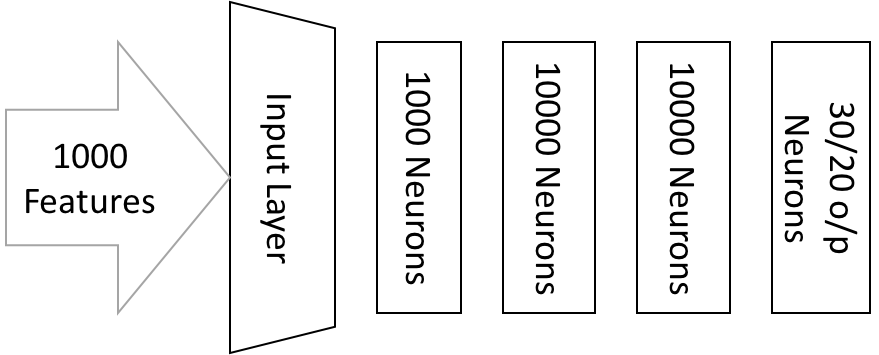
\includegraphics[width=\columnwidth]{figures/NN_diag}
\caption{\textbf{ Neural network architecture for vine repost and like predicton }}
\label{fig:NN_diag}
\end{figure}





